\documentclass[../taasin.tex]{subfiles}
\graphicspath{{\subfix{../figures/}}}
\begin{document}

Our goal is to create an SNN that, when used, allows the biomimetic eye to track an object through space. The object of choice is a white ball that moves against a background whose color varies in different shades of grey. The biomimetic eye of \cite{Arjun} has four main parts, one of which we control with a SNN. We test our implementation by checking that our modified eye model performs certain movements with biological accuracy and that it can successfully track the target. In this section we provide more detail about the eye model, focusing on the retina and foveation controller that our work is based on.

This thesis focuses on replacing the foveation controller with a spiking neural network. This is because of the unique object tracking task that it solves.

%********************************************************************%

\subsection{Retina}

Our virtual retina, like a real one, sits at the back of the eye and contains photoreceptors that get input from the scene. We work with color input, so each photoreceptor collects a red, green, and blue color value. The photoreceptors are distributed according to a log-polar distribution whose equation is shown below. This distribution puts most of the photoreceptors in the center of the retina, simulating the fovea which allows for high acuity vision in the center of mammalian  fields of view.

$$
d_k = e^{\rho_j} 
    \begin{bmatrix} 
        cos( \alpha_i) \\ 
        sin( \alpha_i) 
    \end{bmatrix}
    +
    \begin{bmatrix} 
        \mathcal{N}(\mu, \sigma^2) \\ 
        \mathcal{N}(\mu, \sigma^2)
    \end{bmatrix}
    \text{, for }
    1 \leq k \leq 14,400
$$

% cite papers about actual eye structure

We choose to work with 14,400 photoreceptors, incrementing $\rho_j$ and $\alpha_i$ in steps of 1 with the conditions: $ 0 \leq \rho_j \leq 40 $ and $ 0 \leq \alpha_i \leq 360 $. The second term of the equation is additive noise picked IID from a Gaussian distribution with mean $ \mu = 0 $ and variance $ \sigma^2 = 0.0025 $. Having a lower amount of photoreceptors speeds up simulation and training, but the number can be scaled up as human retinas have about about 6 million cones (for color) and 120 million rods (for black and white) \cite{rodsAndCones}. 

\begin{figure}[h]
    \centering
    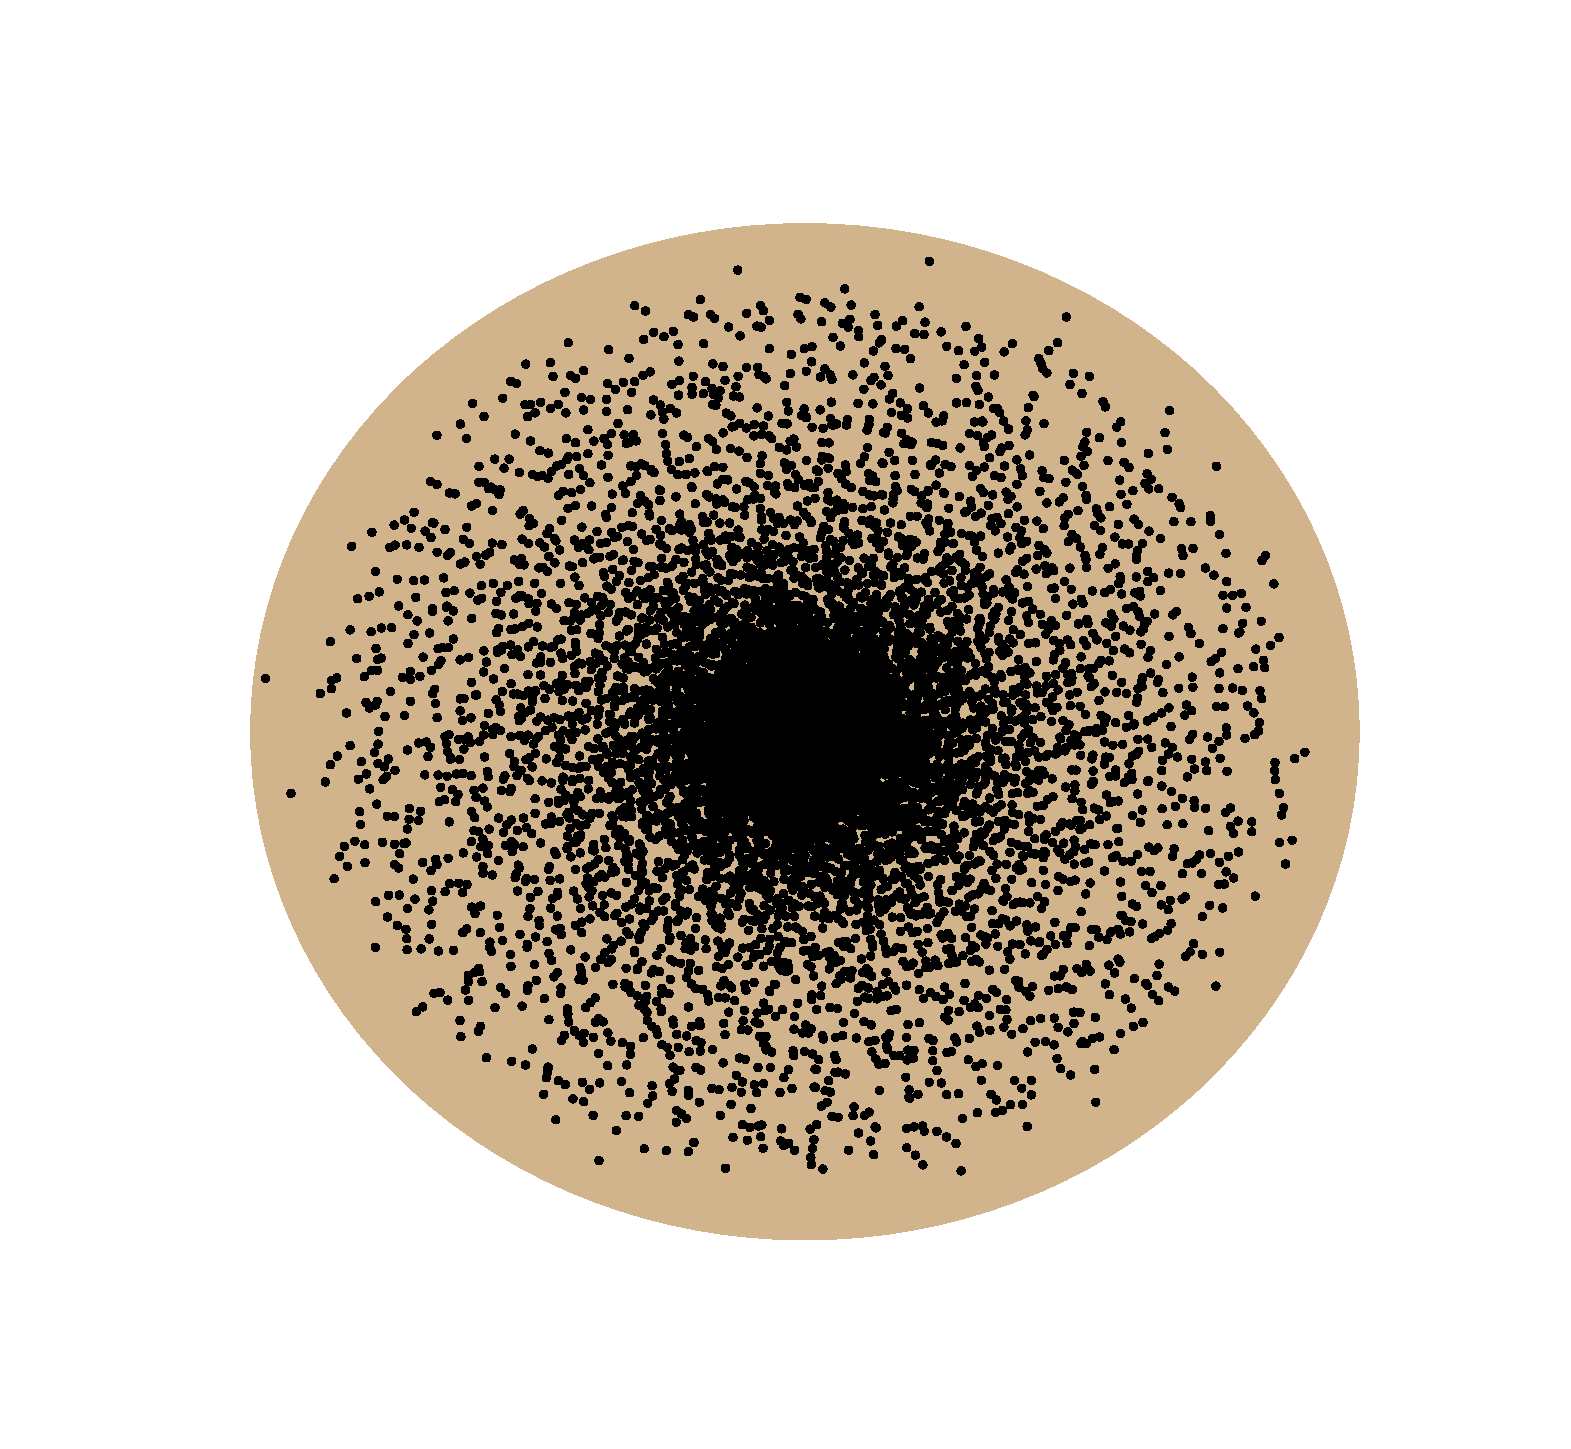
\includegraphics[width=0.6\textwidth]{figures/retina_log_polar.pdf}
    \caption{The photoreceptors of the retina arranged according to a noisy log-polar distribution. The 2D distribution is mapped to the spherical back of the eyeball when ray casting.}
    \label{fig:task_log_polar_retina}
\end{figure}

In our simulation, rays are traced from the retina, through the pupil and lens, to see if they intersect with objects in the scene. These intersections tell us what color will be seen at a given photoreceptor. Therefore, we get 14,400 color intensities. We stack each color channel vertically to create a vector of dimension 43,200. This vector is referred to as the optic nerve vector (ONV).

%********************************************************************%

\subsection{Ocular Organs and Muscles}

The other parts of the eye model include the lens, pupil, and 6 extraocular contractile (EOC) muscles. The pupil and lens help to focus our target onto the retina while the EOC muscles create the movement required for the eye to track the target. Each of these systems is simulated with inverse dynamics control in this thesis; more detail about each subsystem is provided in Appendix \ref{appendix:eye}.

%********************************************************************%

\subsection{Neural Network Controllers}

For added realism and biological performance, each of the ocular organs and muscles can also be controlled with their own neural network. A summary of the whole system is shown in figure \ref{fig:eye controller summary}. The pupil and lens are each controlled with a shallow neural network that takes the ONV as input and outputs one value for the muscle activation.

EOC control is split up into two parts. First the ONV is input to the foveation controller, which takes outputs 2 values $\theta$ and $\phi$. These two values represent the change in the horizontal and vertical directions relative to the eye's current gaze direction. For a target movement such as in figure \ref{fig:2D eye coordinates}, theta is and phi is. This foveation controller is implemented as a locally connected network, dubbed a LiNet. The details of how a LiNet works can be found in \ref{appendix:linet}. The muscle controller then takes these two angles and outputs an activation for each of the EOC muscles to perform the movement.

A summary of the whole system is shown in figure \ref{fig:eye controller summary}.

% \begin{figure}[h]
%     \centering
%     \includegraphics[width=0.5\textwidth]{figures/eye_coordinates.png}
%     \caption{The two angles $\theta$ and $\phi$ needed to describe how the eye must move to follow the target.}
%     \label{fig:2D eye coordinates}
% \end{figure}

\begin{figure}
     \centering
     \begin{subfigure}[b]{0.45\textwidth}
         \centering
         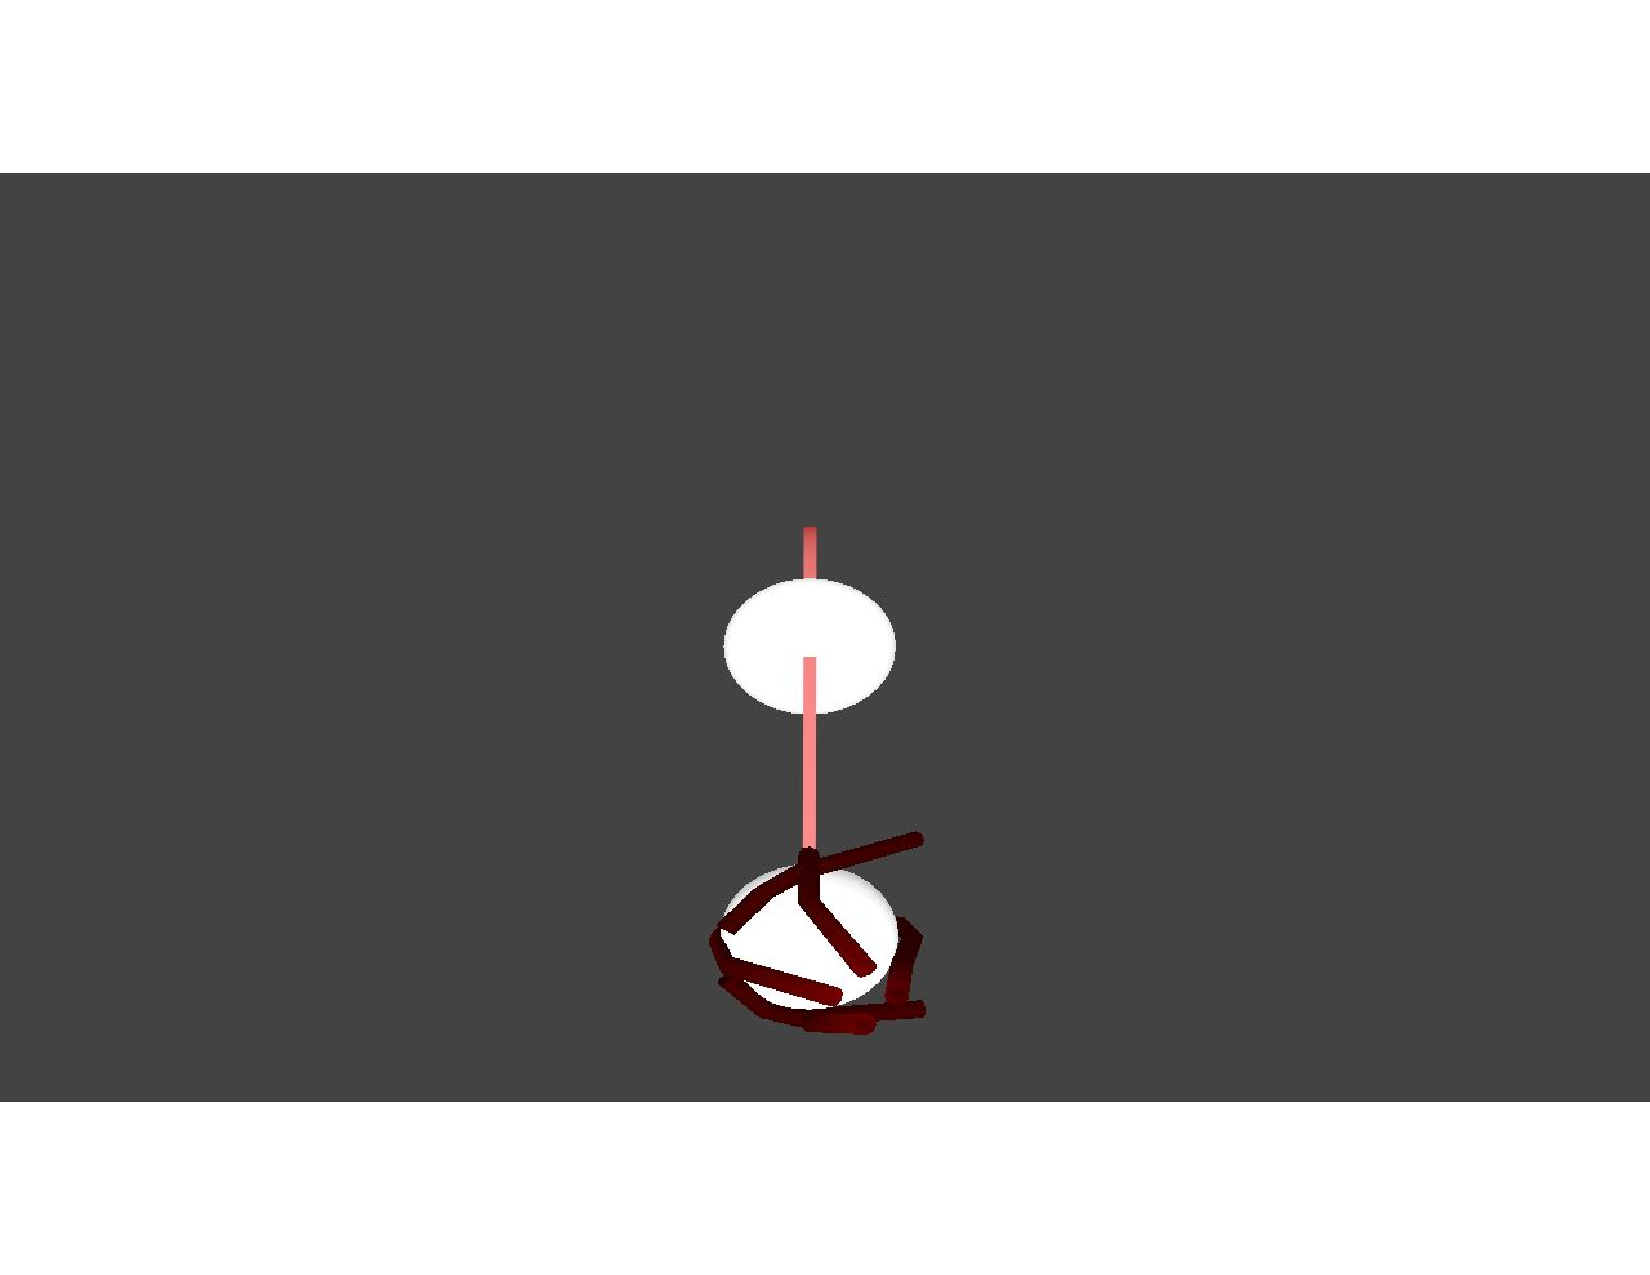
\includegraphics[width=\textwidth]{figures/image000028.pdf}
         \caption{}
         \label{fig:ball_pos1}
     \end{subfigure}
     \hfill
     \begin{subfigure}[b]{0.45\textwidth}
         \centering
         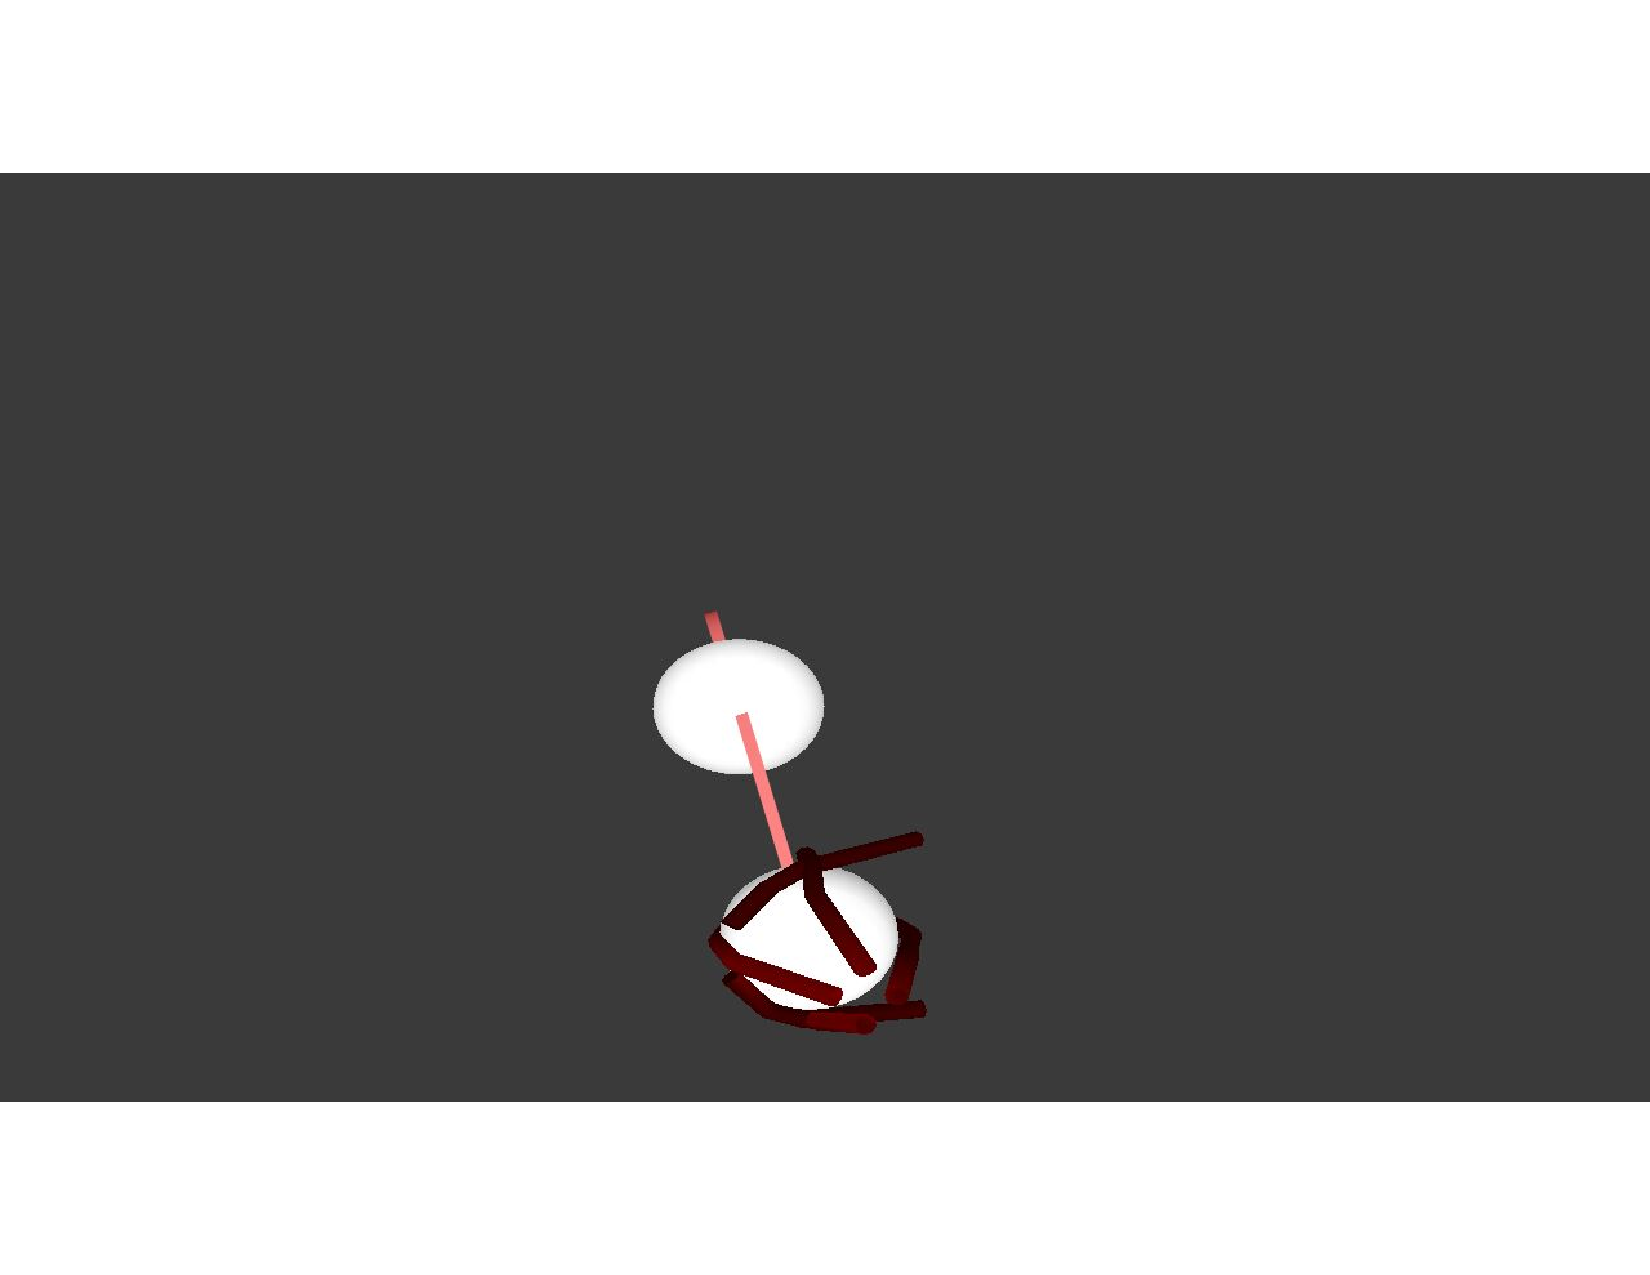
\includegraphics[width=\textwidth]{figures/image000068.pdf}
         \caption{}
         \label{fig:ball_pos2}
     \end{subfigure}
    \caption{Here the ball moves from one point to another. The red line shows the gaze direction, and we can see that the line moves to the left and slightly down. This movement is encoded in the angles theta and phi.  }
    \label{fig:ball_movement}
\end{figure}


% add red box
\begin{figure}[h]
    \centering
    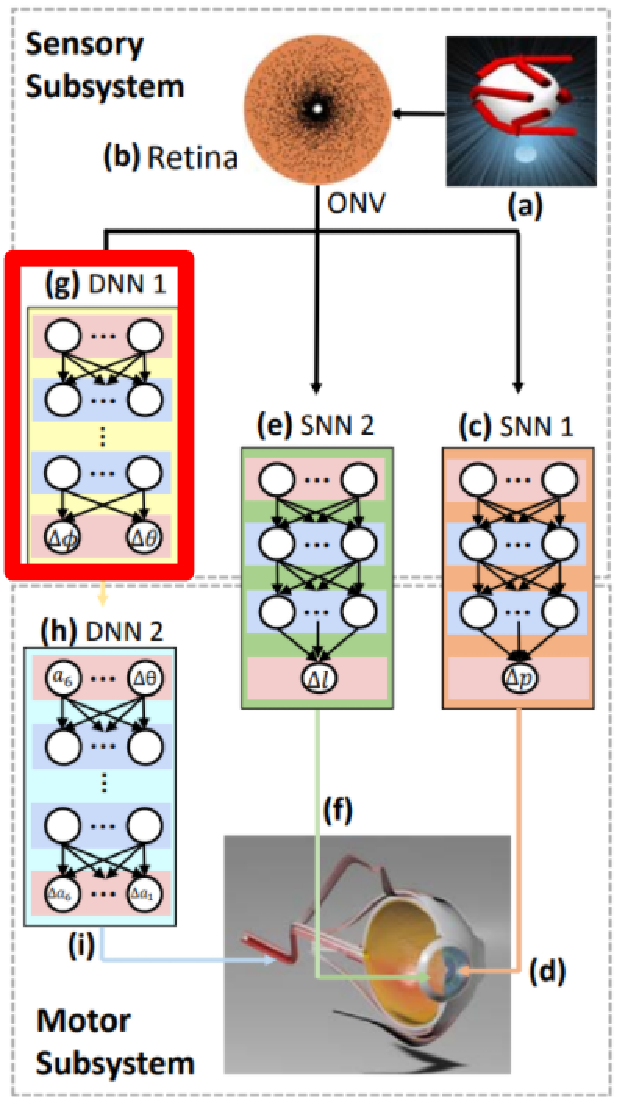
\includegraphics[width=0.5\textwidth]{figures/subsystem_summary2.pdf}
    \caption{Summary of the eye neural network controller system. The foveation controller is highlighted with the red box. Note that SNN in this figure stands for "shallow neural network", not spiking neural network. DNN stands for "deep neural network." Figure from \cite{Arjun}. }
    \label{fig:eye controller summary}
\end{figure}

%********************************************************************%

\subsection{Eye Movements}

We test our SNN foveation controller with the framework created by \cite{Arjun}. This involves moving the target in four different ways, each of which has a different objective that we monitor. The movements are defined below.

\begin{enumerate}
    \item \textit{Saccade}: A quick eye movement to bring a visual target from peripheral vision to the center of the retina. We test that our SNN model matches the angular orientation, velocity, and acceleration of a real eye.
    \item \textit{Fixation}: The eye maintains focus on the target while it stays in place. The eye itself looks still and stable but may have small oscillations. We test that these small oscillations exist as they add to the biological plausibility of the model. 
    \item \textit{Smooth pursuit}: Once a moving visual target is fixated, the eye can pursue the target as it moves. The trajectory of the eye movement is not entirely smooth but includes random oscillation. We track the orientation of the eye through time to make sure that it successfully follows the target. Good performance here is an indication that the eye can track the target through many different trajectories.
    \item \textit{Projectile Motion}: This is similar to smooth pursuit except that the target now changes size as it moves away from the eye. 

We don't test for the vestibulo-ocular reflex (VOR) as we did not have access to the muskuloskeletal model created by \cite{Masaki}. However, we introduce a method to quantitatively evaluate how well our SNNs perform compared to the LiNet.

\end{enumerate}

%%%%%%%%%%%%%%%%%%%%%%%%%%%%%%%%%%%%%%%%%%%%%%%%%%%%%%%%%%%%%%%%%%%%%%

\end{document}